\documentclass[12pt,a4paper] {article}
\usepackage{pgf,tikz}
\usetikzlibrary{calc,intersections,through,backgrounds}

\begin{document}

\begin{figure}[htbp]
\centering
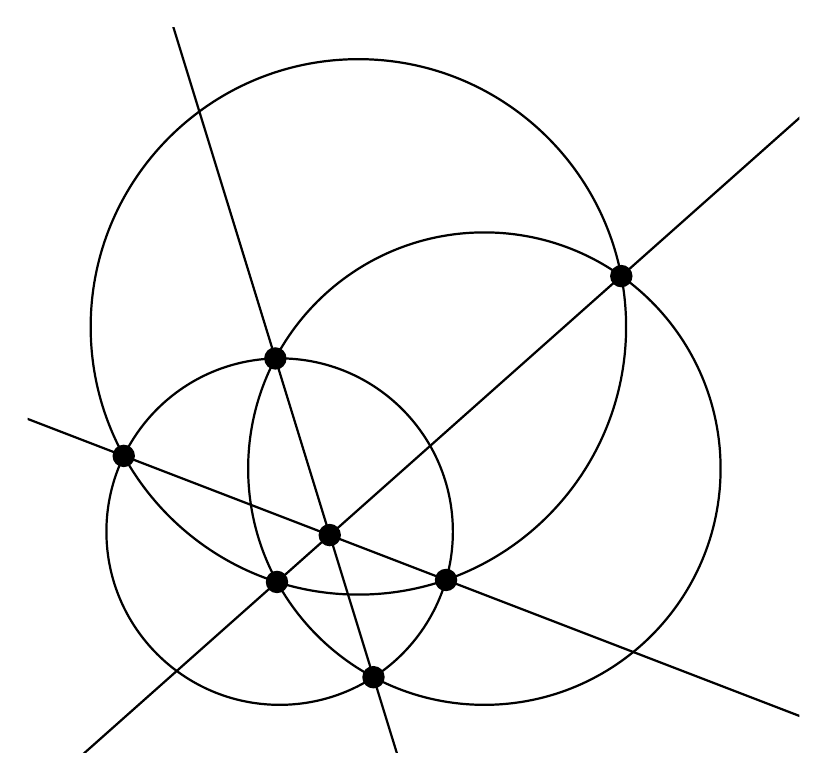
\begin{tikzpicture}[x=2cm,y=2cm]
\tikzset{mainline/.style={thick,color=black}};

\pgfmathsetmacro{\xlo}{-1.1};
\pgfmathsetmacro{\xhi}{3.8};
\pgfmathsetmacro{\ylo}{-1.3};
\pgfmathsetmacro{\yhi}{3.3};
\pgfmathsetmacro{\marg}{.5};
\pgfmathsetmacro{\rone}{1.1};
\pgfmathsetmacro{\rtwo}{1.5};
\pgfmathsetmacro{\rthree}{1.7};
\pgfmathsetmacro{\pointsize}{.0025cm};
\pgfmathsetmacro{\linscale}{20};

\clip (\xlo,\ylo) rectangle (\xhi,\yhi);

\coordinate (A) at (.5,.1);
\coordinate (B) at (1.8,0.5);
\coordinate (C) at (1.,1.4);

\draw [name path=omega_1, mainline] (A) circle (\rone);
\draw [name path=omega_2, mainline] (B) circle (\rtwo);
\draw [name path=omega_3, mainline] (C) circle (\rthree);

\path [name intersections={of=omega_1 and omega_2, by={P_1-2, Q_1-2}}];
\path [name intersections={of=omega_2 and omega_3, by={P_2-3, Q_2-3}}];
\path [name intersections={of=omega_3 and omega_1, by={P_3-1, Q_3-1}}];

\draw [name path=axis_1-2, mainline] ($ (P_1-2)!\linscale!(Q_1-2) $) -- ($ (Q_1-2)!\linscale!(P_1-2) $);
\draw [name path=axis_2-3, mainline] ($ (P_2-3)!\linscale!(Q_2-3) $) -- ($ (Q_2-3)!\linscale!(P_2-3) $);
\draw [name path=axis_3-1, mainline] ($ (P_3-1)!\linscale!(Q_3-1) $) -- ($ (Q_3-1)!\linscale!(P_3-1) $);

\path [name intersections={of=axis_1-2 and axis_2-3, by=C}];

\fill (P_1-2) circle (\pointsize);
\fill (Q_1-2) circle (\pointsize);
\fill (P_2-3) circle (\pointsize);
\fill (Q_2-3) circle (\pointsize);
\fill (P_3-1) circle (\pointsize);
\fill (Q_3-1) circle (\pointsize);
\fill (C) circle (\pointsize);
\end{tikzpicture}
\end{figure}

\end{document}
